%\documentclass{book}
\documentclass{report}

\pagenumbering{roman} 
\pagestyle{empty}

% Notas de aula
%
% Template criado em 24/9/2013
% Daniel Oliveira Dantas
%
% Ctrl+x 8 , c = ç

\usepackage[utf8]{inputenc}
\usepackage[english, brazil]{babel}

\usepackage{listings}
\lstset{
  language=C,                     % choose the language of the code
  numbers=none,                   % where to put the line-numbers
  stepnumber=1,                   % the step between two line-numbers.        
  numbersep=10pt,                 % how far the line-numbers are from the code
  %backgroundcolor=\color{white}, % choose the background color. You must add \usepackage{color}
  showspaces=false,               % show spaces adding particular underscores
  showstringspaces=false,         % underline spaces within strings
  showtabs=false,                 % show tabs within strings adding particular underscores
  tabsize=2,                      % sets default tabsize to 2 spaces
  captionpos=b,                   % sets the caption-position to bottom
  breaklines=true,                % sets automatic line breaking
  breakatwhitespace=true,         % sets if automatic breaks should only happen at whitespace
  title=\lstname,                 % show the filename of files included with \lstinputlisting;
}

% Adicionado para permitir a criação de listas com vários graus de aninhamento
% ddantas, 24/03/2020
\usepackage{amssymb}
\usepackage{amsmath}
\usepackage[ampersand]{easylist}
\ListProperties(Hide=100, Hang=true, Progressive=3ex, Style*=--- ,
Style2*=$\bullet$ ,Style3*=$\circ$ ,Style4*=\tiny$\blacksquare$ )

% Adicionado para permitir a inserção de figuras
% ddantas, 24/03/2020
\usepackage{graphicx}

% Adicionado para permitir a inserção de figuras
% ddantas, 31/03/2020
\usepackage{subcaption}

%formatacao

\newcommand{\TAB}{{\hspace*{1cm}}}
\newcommand{\NEWLINE}{~\\}
\newcommand{\BV}{\begin{verbatim}}
\newcommand{\EV}{\end{verbatim}}

%tipos de dados

\newcommand{\VOID}{{\tt void}}
\newcommand{\CHAR}{{\tt char}}
\newcommand{\INT}{{\tt int}}
\newcommand{\FLOAT}{{\tt float}}
\newcommand{\DOUBLE}{{\tt double}}

\newcommand{\LONGINT}{{\tt long int}}

%operadores

%\newcommand{\AND}{{\tt \&\&}}
%\newcommand{\OR}{{\tt ||}}

%\newcommand{\LNOT}{{\tt \~{}}}
%\newcommand{\LAND}{{\tt \&}}
%\newcommand{\LOR}{{\tt |}}
%\newcommand{\LXOR}{{\tt \^{}}}

%palavras reservadas

\newcommand{\IF}{{\tt if}}
\newcommand{\ELSE}{{\tt else}}

\newcommand{\SWITCH}{{\tt switch}}
\newcommand{\CASE}{{\tt case}}

\newcommand{\FOR}{{\tt for}}
\newcommand{\WHILE}{{\tt while}}

\newcommand{\BREAK}{{\tt break}}

%\newcommand{\TRUE}{{\tt true}}
%\newcommand{\FALSE}{{\tt false}}

\newcommand{\MAIN}{{\tt main}}

\newcommand{\SIZEOF}{{\tt sizeof}}

% funcoes

\newcommand{\SIN}{{\tt sin}}
\newcommand{\COS}{{\tt cos}}
\newcommand{\TAN}{{\tt tan}}
\newcommand{\LOG}{{\tt log}}

\newcommand{\PRINTF}{{\tt printf}}
\newcommand{\SCANF}{{\tt scanf}}

\newcommand{\SPRINTF}{{\tt sprintf}}
\newcommand{\SSCANF}{{\tt sscanf}}

\newcommand{\FPRINTF}{{\tt fprintf}}
\newcommand{\FSCANF}{{\tt fscanf}}

\newcommand{\GETS}{{\tt gets}}
\newcommand{\FGETS}{{\tt fgets}}

\newcommand{\FOPEN}{{\tt fopen}}
\newcommand{\FCLOSE}{{\tt fclose}}

\newcommand{\SYSTEM}{{\tt system}}

% outros

\newcommand{\source}[1]{  \vspace{-6pt}  \caption*{ \footnotesize{Fonte: {#1}} }  }
\newcommand{\ind}{\hspace{1cm}}
\newcommand{\DFT}{\mathfrak{F}}
\newcommand{\IFT}{\mathfrak{F}^{-1}}

% lógica

\newcommand{\NOT}{\sim}
\newcommand{\OR}{\lor}
\newcommand{\AND}{\land}
\newcommand{\NAND}{\barwedge}
\newcommand{\IMP}{\rightarrow}
\newcommand{\BIC}{\leftrightarrow}
\newcommand{\DIMP}{\Rightarrow}
\newcommand{\DBIC}{\Leftrightarrow}
\newcommand{\ISINT}{\vdash}
\newcommand{\ISEM}{\vDash}
\newcommand{\TRUE}{\textit{true}}
\newcommand{\FALSE}{\textit{false}}

\newcommand{\QED}{\blacksquare}

\newcommand{\COMP}{\operatorname{comp}}

\newcommand{\SKIP}{\vspace{0.5cm}}

%renewcommand

\renewcommand\chaptername{Capítulo}
\renewcommand\lstlistingname{Listagem}
%\renewcommand\editionname{Edição}


\title{Notas de aula de Lógica para Ciência da Computação}
\author{Daniel Oliveira Dantas}
\date{11 de setembro de 2020}
\begin{document}

\maketitle

%%%%%%%%%%%%%%%%%%%%%%%%%%%%%%%%%%%%%%%%%%%%%%%%%%%%%%%%%%%%
%Índice
%%%%%%%%%%%%%%%%%%%%%%%%%%%%%%%%%%%%%%%%%%%%%%%%%%%%%%%%%%%%

\tableofcontents
\pagestyle{plain}


%%%%%%%%%%%%%%%%%%%%%%%%%%%%%%%%%%%%%%%%%%%%%%%%%%%%%%%%%%%%
%Capítulo: A linguagem da lógica proposicional
%%%%%%%%%%%%%%%%%%%%%%%%%%%%%%%%%%%%%%%%%%%%%%%%%%%%%%%%%%%%

\chapter{A linguagem da lógica proposicional}


\setcounter{page}{1}    % set page to 1 again to start arabic count
\pagenumbering{arabic}


Capítulo 1 de Souza, \textit{Lógica para Ciência da Computação}~\cite{souza_logica_3}.

\vspace{1cm}

%%%%%%%%%%%%%%%%%%%%%%%%%%%%%%%%%%%%%%%%%%%%%%%%%%%%%%%%%%%%
\begin{easylist}
  & Alfabeto: o alfabeto da Lógica Proposicional é composto por
  && Símbolos de pontuação: $( \; )$
  && Símbolos de verdade: $\TRUE \; \FALSE$
  && Símbolos proposicionais: $A \; B \; C \; P \; Q \; R \; A_1 \; A_2 \; A_3 \; a \; b \; c \; \dots$
  &&& Não se usam as letras $V, v, F, f, T$ e $t$ para não confundir com os valores de verdade.
  && Conectivos proposicionais: $ \NOT \; \OR \; \AND \; \IMP \; \BIC$

\SKIP
  
  & Fórmula: as fórmulas da linguagem da lógica proposicional são construídas a partir dos símbolos do alfabeto conforme as regras a seguir:
  && Todo símbolo de verdade é uma fórmula.
  && Todo símbolo proposicional é uma fórmula.
  && Se $H$ é fórmula, $\NOT H$ é fórmula.
  && Se $H$ e $G$ são fórmulas, $(H \OR G)$, $(H \AND G)$, $(H \IMP G)$ e $(H \BIC G)$ são fórmulas.

\SKIP
  
  & Fórmulas mal formadas: são fórmulas não obtidas da definição anterior.

\SKIP
  
  & Ordem de precedência:
  && $\NOT$      \hspace{2.4cm} Precedência maior.
  && $\IMP \BIC$ \hspace{2cm} $A \IMP B \BIC C$ possui duas interpretações.
  && $\AND$
  && $\OR$       \hspace{2.5cm} Precedência menor.

\SKIP
\SKIP
\SKIP
  
  & Comprimento de uma fórmula:
  && Se $H$ é um símbolo proposicional ou de verdade, $\COMP(H) = 1$.
  && Se $H$ é fórmula, $\COMP(\NOT H) = \COMP(H) + 1$.
  && Se $H$ e $G$ são fórmulas:
  &&& $\COMP(H \OR  G) = \COMP(H) + \COMP(G) + 1$.
  &&& $\COMP(H \AND G) = \COMP(H) + \COMP(G) + 1$.
  &&& $\COMP(H \IMP G) = \COMP(H) + \COMP(G) + 1$.
  &&& $\COMP(H \BIC G) = \COMP(H) + \COMP(G) + 1$.

\SKIP
  
  & Subfórmulas:
  && $H$ é subfórmula de $H$.
  && Se $H = \NOT G$, $G$ é subfórmula de $H$.
  && Se $H$ é uma fórmula do tipo $(G \OR E)$, $(G \AND E)$, $(G \IMP E)$ ou $(G \BIC E)$, então $G$ e $E$ são subfórmulas de $H$.
  && Se $G$ é subfórmula de $H$, então toda subfórmula de $G$ é subfórmula de $H$.

\end{easylist}

%%%%%%%%%%%%%%%%%%%%%%%%%%%%%%%%%%%%%%%%%%%%%%%%%%%%%%%%%%%%
%\section{Componentes de um sistema de processamento de imagens}



%%%%%%%%%%%%%%%%%%%%%%%%%%%%%%%%%%%%%%%%%%%%%%%%%%%%%%%%%%%%
%Capítulo: A semântica da lógica proposicional
%%%%%%%%%%%%%%%%%%%%%%%%%%%%%%%%%%%%%%%%%%%%%%%%%%%%%%%%%%%%

\chapter{A semântica da lógica proposicional}


Capítulo 2 de Souza, \textit{Lógica para Ciência da Computação}~\cite{souza_logica_3}.

\vspace{1cm}

%%%%%%%%%%%%%%%%%%%%%%%%%%%%%%%%%%%%%%%%%%%%%%%%%%%%%%%%%%%%
\begin{easylist}
  & Função: é uma relação entre dois conjuntos que associa cada elemento do conjunto de entrada a um único elemento do conjunto de saída

\SKIP
  
  & Função binária: é uma função em que seu contradomínio possui apenas dois elementos

\SKIP
  
  & Interpretação $I$ é uma função binária tal que:
  && O domínio de $I$ é constituído pelo conjunto de fórmulas da lógica proposicional.
  && O contradomínio de $I$ é o conjunto $\{T, F\}$.
  && $I(\TRUE) = T,  \; I(\FALSE) = F$.
  && Se $P$ é um símbolo proposicional, $I(P) \in \{T, F\}$.

\SKIP
  
  & Interpretação de fórmulas: dadas uma fórmula $E$ e uma interpretação $I$, o significado ou interpretação de $E$, denotado por $I(E)$, é determinado pelas regras:
  && Se $E = P$, onde $P$ é um símbolo proposicional, então $I(E) = I(P)$, onde $I(P) \in \{T, F\}$.
  && Se $E = \TRUE$,  então $I(E) = I(\TRUE)  = T$.
  && Se $E = \FALSE$, então $I(E) = I(\FALSE) = F$.
  && Seja $H$ uma fórmula, se $E = \NOT H$ então:
  &&& $I(E) = I(\NOT H) = T \DBIC I(H) = F$.
  &&& $I(E) = I(\NOT H) = F \DBIC I(H) = T$.

\SKIP

  && Sejam $H$ e $G$ duas fórmulas, se $E = (H \OR G)$ então:
  &&& $I(H) = T$ e/ou   $I(G) = T \DBIC I(E) = I(H \OR G) = T$.
  &&& $I(H) = F$ \;e\;  $I(G) = F \DBIC I(E) = I(H \OR G) = F$.
  && Sejam $H$ e $G$ duas fórmulas, se $E = (H \AND G)$ então:
  &&& $I(H) = T$ \;e\;  $I(G) = T \DBIC I(E) = I(H \AND G) = T$.
  &&& $I(H) = F$ e/ou   $I(G) = F \DBIC I(E) = I(H \AND G) = F$.
  && Sejam $H$ e $G$ duas fórmulas, se $E = (H \IMP G)$ então:
  &&& $I(H) = T$ então  $I(G) = T \DBIC I(E) = I(H \IMP G) = T$.
  &&& $I(H) = F$ e/ou   $I(G) = T \DBIC I(E) = I(H \IMP G) = T$.
  &&& $I(H) = T$ \;e\;  $I(G) = F \DBIC I(E) = I(H \IMP G) = F$.
  && Sejam $H$ e $G$ duas fórmulas, se $E = (H \BIC G)$ então:
  &&& $I(H) =    I(G) \DBIC I(E) = I(H \BIC G) = T$.
  &&& $I(H) \neq I(G) \DBIC I(E) = I(H \BIC G) = F$.

\SKIP

\end{easylist}

%%%%%%%%%%%%%%%%%%%%%%%%%%%%%%%%%%%%%%%%%%%%%%%%%%%%%%%%%%%%
%\section{Componentes de um sistema de processamento de imagens}



%%%%%%%%%%%%%%%%%%%%%%%%%%%%%%%%%%%%%%%%%%%%%%%%%%%%%%%%%%%%
%Capítulo: A sintaxe da lógica proposicional
%%%%%%%%%%%%%%%%%%%%%%%%%%%%%%%%%%%%%%%%%%%%%%%%%%%%%%%%%%%%

\chapter{Propriedades semânticas da Lógica Proposicional}


Capítulo 3 de Souza, \textit{Lógica para Ciência da Computação}~\cite{souza_logica_3}.

\vspace{1cm}

%%%%%%%%%%%%%%%%%%%%%%%%%%%%%%%%%%%%%%%%%%%%%%%%%%%%%%%%%%%%
\section{Propriedades semânticas}

\begin{easylist}
  & Tautologia: uma fórmula $H$ é tautologia ou válida se e somente se (sse) para toda interpretação $I$ \[ I(H) = T \]

\SKIP
  
  & Satisfatibilidade: uma fórmula $H$ é satisfatível ou factível se e somente se (sse) existe pelo menos uma interpretação $I$ tal que \[ I(H) = T \]

\SKIP
  
  & Contingência: uma fórmula $H$ é uma contingência se e somente se (sse) existem interpretações $I$ e $J$ tais que \[ I(H) = T \mbox{ e } J(H) = F \]

\SKIP
  
  & Contradição: uma fórmula $H$ é contraditória se e somente se (sse) para toda interpretação $I$ \[ I(H) = F \]

\SKIP
  
  & Implicação: dadas duas fórmulas $H$ e $G$, $H \ISEM G$ ($H$ implica $G$) sse para toda interpretação $I$ \[ \mbox{ se } I(H) = T \mbox{ então } I(G) = T \]

\SKIP
  
  & Equivalência: dadas duas fórmulas $H$ e $G$, $H$ equivale a $G$ sse para toda interpretação $I$ \[ I(H) = I(G) \]

\SKIP
  
  & Dada uma fórmula $H$ e uma interpretação $I$, dizemos que $I$ satisfaz $H$ se \[ I(H) = T \]

\SKIP
  
  & Um conjunto de fórmulas $\beta = \{H_1, H_2, \dots, H_n\}$ é satisfatível sse existe interpretação $I$ tal que \[ I(H_1) = I(H_2) = \dots = I(H_n) = T \]

\SKIP

  & Um conjunto de fórmulas $\beta = \{H_1, H_2, \dots, H_n\}$ é insatisfatível sse não existe interpretação $I$ tal que \[ I(H_1) = I(H_2) = \dots = I(H_n) = T \]

\end{easylist}

%%%%%%%%%%%%%%%%%%%%%%%%%%%%%%%%%%%%%%%%%%%%%%%%%%%%%%%%%%%%
\section{Relações entre propriedades semânticas}


%%%%%%%%%%%%%%%%%%%%%%%%%%%%%%%%%%%%%%%%%%%%%%%%%%%%%%%%%%%%
%\section{Componentes de um sistema de processamento de imagens}



%%%%%%%%%%%%%%%%%%%%%%%%%%%%%%%%%%%%%%%%%%%%%%%%%%%%%%%%%%%%
%Capítulo: Métodos semânticos de dedução na lógica proposicional
%%%%%%%%%%%%%%%%%%%%%%%%%%%%%%%%%%%%%%%%%%%%%%%%%%%%%%%%%%%%

\chapter{Métodos semânticos de dedução na lógica proposicional}


Capítulo 4 de Souza, \textit{Lógica para Ciência da Computação}~\cite{souza_logica_3}.

\vspace{1cm}


%%%%%%%%%%%%%%%%%%%%%%%%%%%%%%%%%%%%%%%%%%%%%%%%%%%%%%%%%%%%
\section{Introdução}

\begin{easylist}
  & Validade de fórmulas: uma fórmula é válida sse todas as suas interpretações são iguais a $V$.
\end{easylist}


%%%%%%%%%%%%%%%%%%%%%%%%%%%%%%%%%%%%%%%%%%%%%%%%%%%%%%%%%%%%
\section{Método da tabela verdade}

\begin{easylist}
  & Método da tabela verdade: é um método exaustivo, ou seja, enumera todas as possibilidades. A desvantagem é que, se houver muitos símbolos proposicionais, a tabela fica muito grande.
  & Exemplo: seja $H = \; \NOT(P \AND Q) \BIC (\NOT P \OR \NOT Q)$, demonstre que $H$ é uma tautologia usando o método da tabela verdade.  
\end{easylist}

\begin{center}
  \begin{tabular}{ c|c|c|c|c|c|c|c }
    $P$ & $Q$ & $\NOT P$ & $\NOT Q$ & $(P \AND Q)$ & $\NOT(P \AND Q)$ & $(\NOT P \OR \NOT Q)$ & $H$ \\
    \hline
    $T$ & $T$ & $F$      & $F$      & $T$          & $F$              & $F$                   & $T$ \\
    $T$ & $F$ & $F$      & $T$      & $F$          & $T$              & $T$                   & $T$ \\
    $F$ & $T$ & $T$      & $F$      & $F$          & $T$              & $T$                   & $T$ \\
    $F$ & $F$ & $T$      & $T$      & $F$          & $T$              & $T$                   & $T$ \\
  \end{tabular}
\end{center}

%%%%%%%%%%%%%%%%%%%%%%%%%%%%%%%%%%%%%%%%%%%%%%%%%%%%%%%%%%%%
\section{Método da árvore semântica}

\begin{easylist}
  & Método da árvore semântica: é um método que permite a verificação da validade de uma fórmula sem ser exaustivo. A depender da fórmula, pode ser possível obter a resposta sem verificar todas as interpretações possíveis.
  
  & Exemplo: seja $H = \; \NOT(P \AND Q) \BIC (\NOT P \OR \NOT Q)$, demonstre que $H$ é uma tautologia usando o método da árvore semântica.
\end{easylist}

\begin{center}
  \begin{tabular}{ c|cccccccccc }
        & $\NOT$ & $(P$ & $\AND$ & $Q)$ & $\BIC$ & $(\NOT$ & $P$ & $\OR$ & $\NOT$ & $Q)$ \\
    \hline
      2 &        & $T$  &        &      &        & $F$     & $T$ &       &        &      \\
    \hline
      3 & $T$    & $F$  & $F$    &      & $T$    & $T$     & $F$ & $T$   &        &      \\
    \hline
      4 & $F$    & $T$  & $T$    & $T$  & $T$    & $F$     & $T$ & $F$   & $F$    & $T$  \\
    \hline
      5 & $T$    & $T$  & $F$    & $F$  & $T$    & $F$     & $T$ & $T$   & $T$    & $F$  \\
  \end{tabular}
\end{center}

\begin{figure}[!h]
  \begin{center}
    \begin{tabular}{c}
      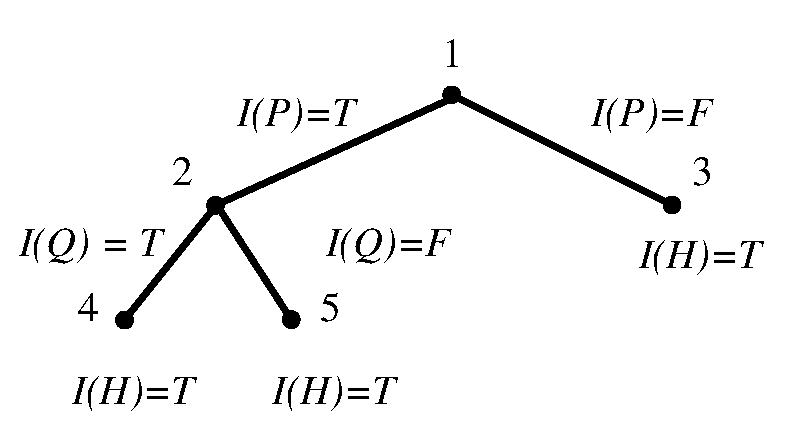
\includegraphics[width=0.7\textwidth]{images/04/tree_01.eps}
    \end{tabular}
  \end{center}
  %\caption{\label{fig:tree:01}}
\end{figure}

\clearpage

\begin{easylist}
  & Exemplo: seja $H = \; (P \OR \NOT Q) \BIC (\NOT P \IMP \NOT Q)$, demonstre que $H$ é uma tautologia usando o método da árvore semântica.
\end{easylist}

\begin{center}
  \begin{tabular}{ c|cccccccccc }
        & $(P$ & $\OR$ & $\NOT$ & $Q)$ & $\BIC$ & $(\NOT$ & $P$ & $\IMP$ & $\NOT$ & $Q)$ \\
    \hline
      2 & $T$  & $T$   &        &      & $T$    & $F$     & $T$ & $T$    &        &      \\
    \hline
      3 & $F$  &       &        &      &        & $T$     & $F$ &        &        &      \\
    \hline
      4 & $F$  & $F$   & $F$    & $T$  & $T$    & $T$     & $F$ & $F$    & $F$    & $T$  \\
    \hline
      5 & $F$  & $T$   & $T$    & $F$  & $T$    & $T$     & $F$ & $T$    & $T$    & $F$  \\
  \end{tabular}
\end{center}

\begin{figure}[!h]
  \begin{center}
    \begin{tabular}{c}
      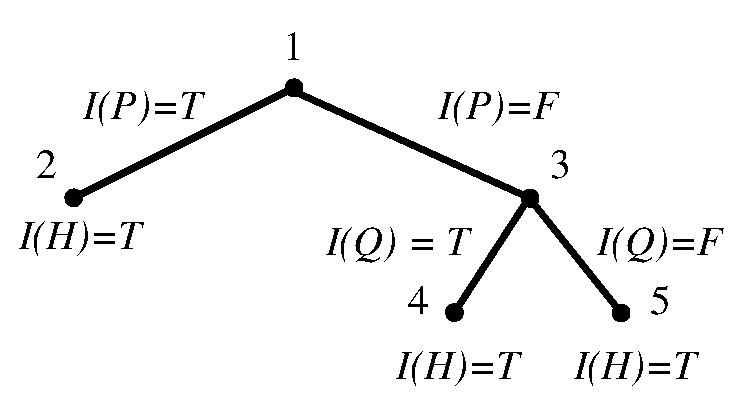
\includegraphics[width=0.7\textwidth]{images/04/tree_02.eps}
    \end{tabular}
  \end{center}
  %\caption{\label{fig:tree:01}}
\end{figure}





%%%%%%%%%%%%%%%%%%%%%%%%%%%%%%%%%%%%%%%%%%%%%%%%%%%%%%%%%%%%
%Capítulo: Um método sintático de dedução na lógica proposicional
%%%%%%%%%%%%%%%%%%%%%%%%%%%%%%%%%%%%%%%%%%%%%%%%%%%%%%%%%%%%

%\chapter{Um método sintático de dedução na lógica proposicional}


Capítulo 5 de Souza, \textit{Lógica para Ciência da Computação}~\cite{souza_logica_3}.

\vspace{1cm}


%%%%%%%%%%%%%%%%%%%%%%%%%%%%%%%%%%%%%%%%%%%%%%%%%%%%%%%%%%%%
\section{Introdução}

\begin{easylist}
  & 
\end{easylist}


%%%%%%%%%%%%%%%%%%%%%%%%%%%%%%%%%%%%%%%%%%%%%%%%%%%%%%%%%%%%
\section{O sistema formal Pa}

\begin{easylist}
  &
\end{easylist}





%%%%%%%%%%%%%%%%%%%%%%%%%%%%%%%%%%%%%%%%%%%%%%%%%%%%%%%%%%%%
%Capítulo: A linguagem da lógica de predicados
%%%%%%%%%%%%%%%%%%%%%%%%%%%%%%%%%%%%%%%%%%%%%%%%%%%%%%%%%%%%

%\chapter{A linguagem da lógica de predicados}


Capítulo 6 de Souza, \textit{Lógica para Ciência da Computação}~\cite{souza_logica_3}.

\vspace{1cm}


%%%%%%%%%%%%%%%%%%%%%%%%%%%%%%%%%%%%%%%%%%%%%%%%%%%%%%%%%%%%
\section{O alfabeto da lógica de predicados}

\begin{easylist}
  & Alfabeto: o alfabeto da lógica de predicados é composto por
  && Símbolos de pontuação: $( \; )$
  && Símbolos de verdade: $\TRUE \; \FALSE$
  && Símbolos para variáveis: $x \; y \; z \; w \; x_1 \; y_1 \; z_1 \; x_2 \dots$
  && Símbolos para funções: $f \; g \; h \; f_1 \; g_1 \; h_1 \; f_2 \dots$
  && Símbolos para predicados: $p \; q \; r \; s \; p_1 \; q_1 \; r_1 \; s_1 \; p_2 \dots$
  && Conectivos: $ \NOT \; \OR \; \AND \; \IMP \; \BIC \; \FA \; \EX$

  & Associado a cada função ou predicado está um número inteiro $k\geq0$ que indica a sua ``aridade'', ou seja, seu número de argumentos.

  & Os símbolos para funções zero-árias, isto é, funções constantes, são: $a \; b \; c \; a_1 \; b_1 \; c_1 \; a_2 \dots$

  & Os símbolos para predicados zero-ários, isto é, símbolos proposicionais, são: $P \; Q \; R \; S \; P_1 \; Q_1 \; R_1 \; S_1 \; P_2 \dots$

\end{easylist}


%%%%%%%%%%%%%%%%%%%%%%%%%%%%%%%%%%%%%%%%%%%%%%%%%%%%%%%%%%%%
\section{Fórmulas da lógica de predicados}

\begin{easylist}
  & Termo: um termo pode ser
  && uma variável
  && $f(t_1, \dots, t_n)$ onde $f$ é uma função $n$-ária e $t_1, \dots, t_n$ são termos.

\SKIP
  A INTERPRETAÇÃO DE UM TERMO É UM OBJETO MATEMÁTICO
\SKIP

  & Átomo: um átomo pode ser
  && um símbolo de verdade
  && $p(t_1, \dots, t_n)$ onde $p$ é um predicado $n$-ário e $t_1, \dots, t_n$ são termos.

\SKIP
  A INTERPRETAÇÃO DE UM ÁTOMO É UM VALOR DE VERDADE $\in \{T, F\}$
\SKIP

  
  & Fórmula: as fórmulas da linguagem da lógica de predicados são construídas a partir dos símbolos do alfabeto conforme as regras a seguir:
  && Todo átomo é uma fórmula.
  && Se $H$ é fórmula, $\NOT H$ é fórmula.
  && Se $H$ e $G$ são fórmulas, então $(H \OR G)$, $(H \AND G)$, $(H \IMP G)$ e $(H \BIC G)$ são fórmulas.
  && Se $H$ é fórmula e $x$ é variável, então, $((\FA x) H)$ e $((\EX x) H)$ são fórmulas.

  & Expressão: uma expressão pode ser
  && um termo
  && uma fórmula

\end{easylist}

%%%%%%%%%%%%%%%%%%%%%%%%%%%%%%%%%%%%%%%%%%%%%%%%%%%%%%%%%%%%
\section{Correspondência entre quantificadores}

\begin{easylist}
  & $ ((\FA x) H) \;\; \equiv \;\; \NOT((\EX x)(\NOT H)) $
  & $ ((\EX x) H) \;\; \equiv \;\; \NOT((\FA x)(\NOT H)) $
\end{easylist}


%%%%%%%%%%%%%%%%%%%%%%%%%%%%%%%%%%%%%%%%%%%%%%%%%%%%%%%%%%%%
\section{Símbolos de pontuação}

\begin{easylist}
  & Ordem de precedência:
  && $\NOT$      \hspace{5cm} Maior
  && $\FA \; \EX$
  && $\IMP \; \BIC$ \hspace{1cm} $A \IMP B \BIC C$ possui duas interpretações.
  && $\AND$
  && $\OR$       \hspace{5cm} Menor
\end{easylist}



%%%%%%%%%%%%%%%%%%%%%%%%%%%%%%%%%%%%%%%%%%%%%%%%%%%%%%%%%%%%
\section{Características sintáticas das fórmulas}

\begin{easylist}

  & Subtermo, subfórmula e subexpressão:
  && Se $E = x$ então x é subtermo de $E$.
  && Se $E = f(t_1, \dots, t_n)$ então $t_1, \dots, t_n, f(t_1, \dots, t_n)$ são subtermos de $E$.
  && Se $H$ é fórmula, $H$ é subfórmula de $H$.
  && Se $E = \NOT H$, então $H$ e $\NOT H$ são subfórmulas de $E$.
  && Se $E$ é uma fórmula do tipo $(G \OR H)$, $(G \AND H)$, $(G \IMP H)$ ou $(G \BIC H)$, então $G$ e $H$ são subfórmulas de $E$.
  && Se $E$ é uma fórmula do tipo $(\FA x)H$ ou $(\EX x)H$, então $H$ é subfórmula de $E$.
  && Se $G$ é subfórmula de $H$, então toda subfórmula de $G$ é subfórmula de $H$.
  && Todo subtermo ou subfórmula é também subexpressão.

  & Comprimento de uma fórmula:
  && Se $H$ é um átomo, $\COMP(H) = 1$.
  && Se $H$ é fórmula, $\COMP(\NOT H) = \COMP(H) + 1$.
  && Se $H$ e $G$ são fórmulas:
  &&& $\COMP(H \OR  G) = \COMP(H) + \COMP(G) + 1$.
  &&& $\COMP(H \AND G) = \COMP(H) + \COMP(G) + 1$.
  &&& $\COMP(H \IMP G) = \COMP(H) + \COMP(G) + 1$.
  &&& $\COMP(H \BIC G) = \COMP(H) + \COMP(G) + 1$.
  && Se $H = ((\FA x)G)$ ou $H = ((\EX x)G)$, então $\COMP(H) = \COMP(G) + 1$.

\SKIP
  
\end{easylist}


%%%%%%%%%%%%%%%%%%%%%%%%%%%%%%%%%%%%%%%%%%%%%%%%%%%%%%%%%%%%
\section{Formas normais}

\begin{easylist}
  & Literal: um literal pode ser
  && um átomo
  && a negação de um átomo

  & Forma normal: uma fórmula está na
  && forma normal conjuntiva (FNC) se for uma conjunção $(\AND)$ de disjunções $(\OR)$ de literais
  && forma normal disjuntiva (FND) se for uma disjunção $(\OR)$ de conjunções $(\AND)$ de literais

\end{easylist}


%%%%%%%%%%%%%%%%%%%%%%%%%%%%%%%%%%%%%%%%%%%%%%%%%%%%%%%%%%%%
\section{Classificações de variáveis}

\begin{easylist}


  & Escopo de um quantificador: seja $G$ uma fórmula da lógica de predicados:
  && Se $(\FA x)H$ é uma subfórmula de $G$, então o escopo de $(\FA x)$ em $G$ é a subfórmula $H$.
  && Se $(\EX x)H$ é uma subfórmula de $G$, então o escopo de $(\EX x)$ em $G$ é a subfórmula $H$.

  \clearpage
  \EXERCICIOS
  \begin{enumerate}
  \item Considere a fórmula abaixo.
    \[ G = (\FA x)(\EX y)((\FA z)p(x,y,z,w) \IMP (\FA y)q(z,y,x,z_1)) \]
    Qual é o escopo de
    \begin{enumerate}
      \item $(\FA x)$
      \item $(\EX y)$
      \item $(\FA z)$
      \item $(\FA y)$
    \end{enumerate}
  \end{enumerate}

  & Ocorrência livre e ligada: sejam $x$ uma variável e $G$ uma fórmula.
  && Uma ocorrência de $x$ em $G$ é ligada se $x$ está no escopo de um quantificador $(\FA x)$ ou $(\EX x)$.
  && Uma ocorrência de $x$ em $G$ é livre se não for ligada.

  & Variável livre e ligada: sejam  $x$ uma variável e $G$ uma fórmula.
  && A variável $x$ é ligada em $G$ se existe pelo menos uma ocorrência ligada de $x$ em $G$.
  && A variável $x$ é livre em $G$ se existe pelo menos uma ocorrência livre de $x$ em $G$.

  & Símbolo livre: seja $G$ uma fórmula, os seus símbolos livres são as variáveis com ocorrência livre em $G$, símbolos de função e símbolos de predicado.

  & Fórmula fechada: uma fórmula é fechada quando não possui variáveis livres.

  & Fecho de uma fórmula: seja $H$ uma fórmula da lógica de predicados, e $\{x_1, \dots, x_n\}$ o conjunto das variáveis livres de $H$.
  && O fecho universal de $H$, indicado por $(\FA *)H$, é dado pela fórmula\\ $(\FA x_1)(\FA x_2)\dots(\FA x_n)H$.
  && O fecho existencial de $H$, indicado por $(\EX *)H$, é dado pela fórmula $(\EX x_1)(\EX x_2)\dots(\EX x_n)H$.
  
\end{easylist}

%%%%%%%%%%%%%%%%%%%%%%%%%%%%%%%%%%%%%%%%%%%%%%%%%%%%%%%%%%%%
\section{Exercícios}

%$ \NOT \; \OR \; \AND \; \IMP \; \BIC$

\begin{enumerate}
  \item Determine o comprimento das fórmulas a seguir.
    \begin{enumerate}
      \item $H_1 = p(x, y, f(z))$
      \item $H_2 =  (P \OR \NOT Q) \IMP \NOT(q(x, y) \OR r(z))$
      \item $H_3 = (\EX y) r(y) \BIC \NOT (\EX y) P)$
      \item $H_4 = \NOT(p(x, y, z)) \IMP \NOT( (\FA x) (\FA y) (\FA z) p(x, y, z))$
    \end{enumerate}
  \item Determine o conjunto de subespressões das expressões a seguir.
    \begin{enumerate}
      \item $H_1 = p(x, y, f(z))$
      \item $H_2 = g(x, y, f(z))$
      \item $H_3 = (\EX y) r(y) \BIC \NOT (\EX y) P)$
      \item $H_4 = \NOT(p(x, y, z)) \IMP \NOT( (\FA x) (\FA y) (\FA z) p(x, y, z))$
    \end{enumerate}
  \item Verdadeiro ou falso?
    \begin{enumerate}
      \item Toda variável é um termo
      \item Todo termo é uma variável
      \item Toda função é um termo
      \item Todo termo é uma função
      \item Toda variável é um átomo
      \item Todo átomo é uma variável
      \item Todo termo é um átomo
      \item Todo átomo é um termo
      \item Todo termo é uma fórmula
      \item Toda fórmula é um termo
      \item Todo átomo é um literal
      \item Todo literal é um átomo
      \item Todo átomo é uma fórmula
      \item Toda fórmula é um átomo 
      \item Todo literal é uma fórmula
      \item Toda fórmula é um literal 
      \item Toda variável é uma expressão
      \item Toda expressão é uma variável
      \item Todo átomo é uma expressão
      \item Toda expressão é um átomo
      \item Todo literal é uma expressão
      \item Toda expressão é um literal
      \item Todo termo é uma expressão
      \item Toda expressão é um termo
    \end{enumerate}
  \item Indique se os itens abaixo são ou não variáveis, termos, funções, átomos, literais, fórmulas e expressões.
    \begin{enumerate}
      \item $z$
      \item $a$
      \item $P \BIC Q$
      \item $g(x, y, z)$
      \item $p(x, y, z)$
      \item $\NOT P$        
    \end{enumerate}
  \item Escreva uma fórmula equivalente usando o quantificador existencial $\EX$.
    \begin{enumerate}
      \item $H_1 = (\FA x) P$
      \item $H_2 = \;\NOT (\FA x) P)$
      \item $H_3 = (\FA x) \NOT P$
      \item $H_4 = \;\NOT((\FA x) \NOT P)$
    \end{enumerate}
  \item Considere a fórmula $(\FA y) ( (\EX x) \NOT q(x) \AND (\EX y) (\FA z) p(y, z) )$. Qual é o escopo de
    \begin{enumerate}
      \item $(\FA y)$
      \item $(\EX x)$
      \item $(\EX y)$
      \item $(\FA z)$
    \end{enumerate}
  \item Indique o escopo de todos os quantificadores das fórmulas abaixo.
    \begin{enumerate}
      \item $(\FA x) ( \; (\FA z) p(x,y,z) \BIC (\FA y) q(x,y,z) \; )$
      \item $(\FA x) p(x,y,z) \IMP (\FA y) (\EX z) q(x,y,z)$
    \end{enumerate}
  \item Indique se as ocorrências de variáveis nas fórmulas abaixo são livres ou ligadas.
    \begin{enumerate}
      \item $(\FA x) ( \; (\FA z) p(x,y,z, w) \BIC (\FA y) q(x,y,z, z_1) \; )$
      \item $(\FA x) ( \;\; p(x,y,z_1) \IMP (\FA y) (\EX z) ( \; q(w,x,y) \AND (\FA w) r(w,x,z) \; ) \;\; )$
    \end{enumerate}
  \item Indique se as variáveis nas fórmulas da questão anterior são livres ou ligadas.
  \item Encontre o fecho universal e o fecho existencial das fórmulas da questão anterior.

\end{enumerate}





%%%%%%%%%%%%%%%%%%%%%%%%%%%%%%%%%%%%%%%%%%%%%%%%%%%%%%%%%%%%
%Capítulo: A semântica da lógica de predicados
%%%%%%%%%%%%%%%%%%%%%%%%%%%%%%%%%%%%%%%%%%%%%%%%%%%%%%%%%%%%

%\input{07.tex}


%%%%%%%%%%%%%%%%%%%%%%%%%%%%%%%%%%%%%%%%%%%%%%%%%%%%%%%%%%%%
%Capítulo: Propriedades semânticas da lógica de predicados
%%%%%%%%%%%%%%%%%%%%%%%%%%%%%%%%%%%%%%%%%%%%%%%%%%%%%%%%%%%%

%\input{08.tex}


%%%%%%%%%%%%%%%%%%%%%%%%%%%%%%%%%%%%%%%%%%%%%%%%%%%%%%%%%%%%
%Capítulo: Métodos semânticos de dedução na lógica de predicados
%%%%%%%%%%%%%%%%%%%%%%%%%%%%%%%%%%%%%%%%%%%%%%%%%%%%%%%%%%%%

%\input{09.tex}


%%%%%%%%%%%%%%%%%%%%%%%%%%%%%%%%%%%%%%%%%%%%%%%%%%%%%%%%%%%%
%Capítulo: Um método sintático de dedução na lógica de predicados
%%%%%%%%%%%%%%%%%%%%%%%%%%%%%%%%%%%%%%%%%%%%%%%%%%%%%%%%%%%%

%\input{10.tex}


%%%%%%%%%%%%%%%%%%%%%%%%%%%%%%%%%%%%%%%%%%%%%%%%%%%%%%%%%%%%
%Capítulo: Exemplos de programas
%%%%%%%%%%%%%%%%%%%%%%%%%%%%%%%%%%%%%%%%%%%%%%%%%%%%%%%%%%%%

%\chapter{Exemplos de programas}


%%%%%%%%%%%%%%%%%%%%%%%%%%%%%%%%%%%%%%%%%%%%%%%%%%%%%%%%%%%%
%Seção: pause.cpp

%\section{pause.cpp}

%\lstinputlisting[caption=series.cpp]{src/pause.cpp}

%%%%%%%%%%%%%%%%%%%%%%%%%%%%%%%%%%%%%%%%%%%%%%%%%%%%%%%%%%%%
%Seção: ascii.cpp

%\section{ascii.cpp}

%\lstinputlisting[caption=ascii.cpp]{src/ascii.cpp}

%%%%%%%%%%%%%%%%%%%%%%%%%%%%%%%%%%%%%%%%%%%%%%%%%%%%%%%%%%%%
%Seção: dado.cpp

%\section{dado.cpp}

%\lstinputlisting[caption=dado.cpp]{src/dado.cpp}

%%%%%%%%%%%%%%%%%%%%%%%%%%%%%%%%%%%%%%%%%%%%%%%%%%%%%%%%%%%%
%Seção: primos.cpp

%\section{primos.cpp}

%\lstinputlisting[caption=series.cpp]{src/primos.cpp}

%%%%%%%%%%%%%%%%%%%%%%%%%%%%%%%%%%%%%%%%%%%%%%%%%%%%%%%%%%%%
%Seção: series.cpp

%\section{series.cpp}

%\lstinputlisting[caption=series.cpp]{src/series.cpp}




%%%%%%%%%%%%%%%%%%%%%%%%%%%%%%%%%%%%%%%%%%%%%%%%%%%%%%%%%%%%
%Seção: generate.cpp

%\section{generate.cpp}

%\lstinputlisting[caption=generate.cpp]{src/generate.cpp}

%%%%%%%%%%%%%%%%%%%%%%%%%%%%%%%%%%%%%%%%%%%%%%%%%%%%%%%%%%%%
%Seção: ordena.cpp

%\section{ordena.cpp}

%\lstinputlisting[caption=ordena.cpp]{src/ordena.cpp}

\bibliography{refs}
\bibliographystyle{plain}


\end{document}

